\documentclass{senior-design}

%%% Fonts %%%%%%%%%%%%%%%%%%%%%%%%%%%%%%%%%%%%%%%%%%%%%%%%%%%%%%%
\setmonofont[Scale=MatchLowercase]{Consolas}
\setsansfont{Arial}
\usepackage{newpxtext, newpxmath} % Palatino
\graphicspath{{Figures/}}

%%% Report information %%%%%%%%%%%%%%%%%%%%%%%%%%%%%%%%%%%%%%%%%%
\reporttitle{Human-Robot Interaction for Object Grasping with Virtual Reality and Robotic Arms }
\reporttype{Design Document} % Uncomment this line if you want to use \generalreportcover
\semester{Spring 2025}
\sponsor{Prof. \name{Gaoang}{Wang} \& Prof. \name{Liangjing}{Yang}}
\ta{\name{Tielong}{Cai} \& \name{Tianci}{Tang}}
\reportdate{\today}
\authornames{
    \nameemail{Jiayu}{Zhou}{jiayu9@illinois.edu}\\[1em]
    \nameemail{Ziming}{Yan}{zimingy3@illinois.edu}\\[1em]
    \nameemail{Yuchen}{Yang}{yucheny8@example.com}\\[1em]
    \nameemail{Jingxing}{Hu}{hu80@illinois.edu}
}
\projectnumber{26}
\teamnumber{514}
\addbibresource{references.bib} % The bib databas
%%%%%%%%%%%%%%%%%%%%%%%%%%%%%%%%%%%%%%%%%%%%%%%%%%%%%%%%%%%%%%%%%
\begin{document}
%%% TITLE PAGE %%%%%%%%%%%%%%%%%%%%%%%%%%%%%%%%%%%%%%%%%%%%%%%%%%
\generalreportcover % coverpage for other reports; NEEDS \reporttype{<Type>}
%%%%%%%%%%%%%%%%%%%%%%%%%%%%%%%%%%%%%%%%%%%%%%%%%%%%%%%%%%%%%%%%%
\frontmatter
%%% TOC %%%%%%%%%%%%%%%%%%%%%%%%%%%%%%%%%%%%%%%%%%%%%%%%%%%%%%%%%
\tableofcontents
%%%%%%%%%%%%%%%%%%%%%%%%%%%%%%%%%%%%%%%%%%%%%%%%%%%%%%%%%%%%%%%%%

\mainmatter
%%% Body %%%%%%%%%%%%%%%%%%%%%%%%%%%%%%%%%%%%%%%%%%%%%%%%%%%%%%%%
\setstretch{2}
\chapter{Introduction}
Briefly describe the science or engineering problem to be addressed in the report, as well as the purpose and usefulness of the device or system you have built. Summarize the contents of the upcoming chapters as well as the main conclusions of your project, to be elaborated in the last chapter.

\section{Sample equations}
\begin{equation}
    EQI = \sum_{i=1}^{n}W_j * r_{ij}
\end{equation}

\begin{equation}
    EHI = L_1 \times ESI + L_2 \times EQI
\end{equation}

\begin{equation}
    \begin{aligned}
        EE / EHI = \beta_0 & + \beta_1 PCG + \beta_2 RGP + \cdots + \beta_i X_i +              \\
        \cdots             & + \beta_9 ICWUR + \beta_{10} ECPG + \beta_11 WCPG + \varepsilon_i
    \end{aligned}
\end{equation}

\section{Sample listings}
This is a sample listing.
\begin{lstlisting}[language=c]
#include<stdio.h>
void fuzzy(int x){
    return x;
}
int main(){
    int a = 0, b, c;
    scanf("%d", &b);
    c = b;
    if (a == b)
        a = fuzzy(c);
    else
        b = fuzzy(a);
    printf("%d %d\n", a, fuzzy(c));
    return 0;
}
\end{lstlisting}

\chapter{Design}


\section{Block Diagram}
\begin{figure}[H]
    \centering
    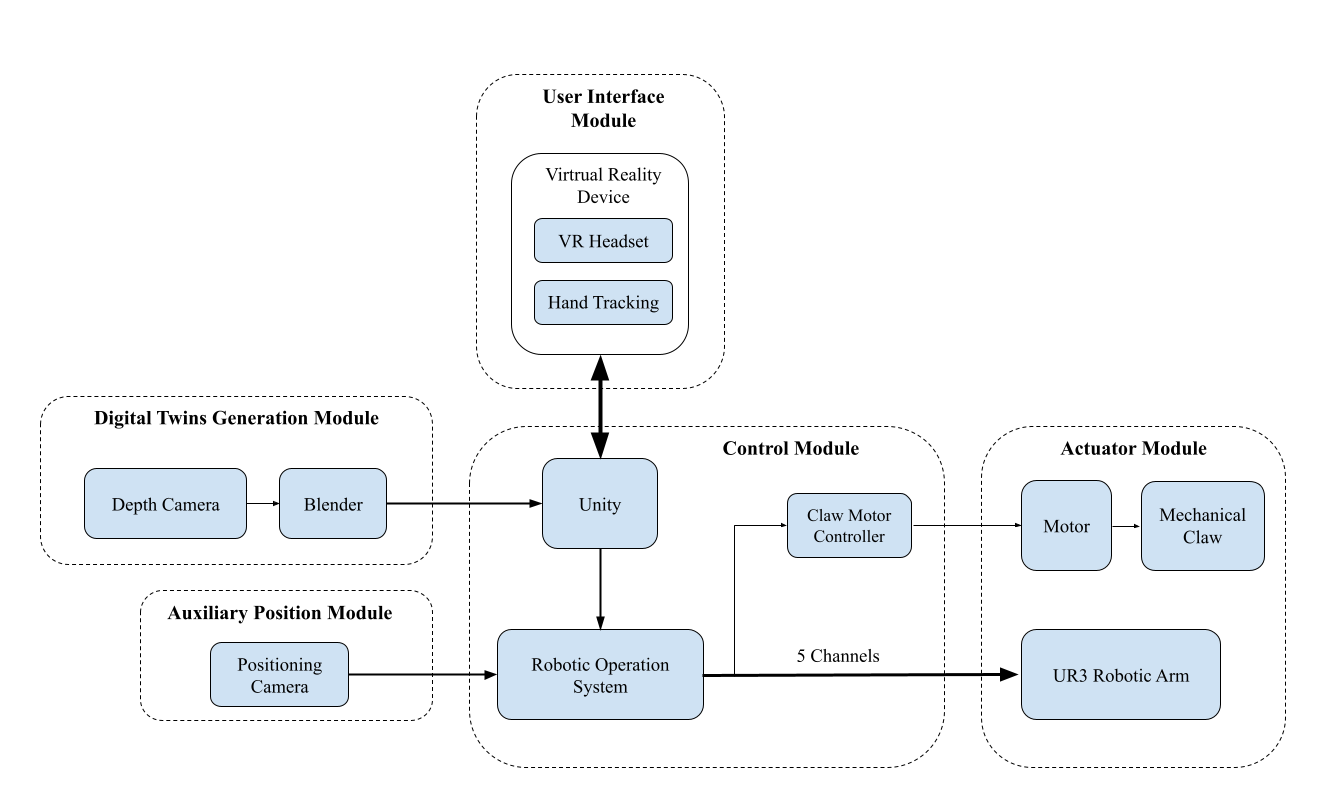
\includegraphics[width=0.9\linewidth]{Block Diagram.png}
    \caption{Block Diagram}
\end{figure}
\section{Physical Design}
Since the original robotic arm realizes picking up and placing objects through 
the suction force of suction cups, this limits the accuracy and fineness of 
gripping objects. Therefore, we decided to create a suitable mechanical claw 
through 3D modeling and control the motor to drive the mechanical claw to clamp
, thus replacing the operation of the suction cup. We believe that this will 
dramatically increase the level of maneuverability and reduce the requirements 
for the material and shape of the object to be gripped. The following figure shows
our design model of claw.
\begin{figure}[H]
    \centering
    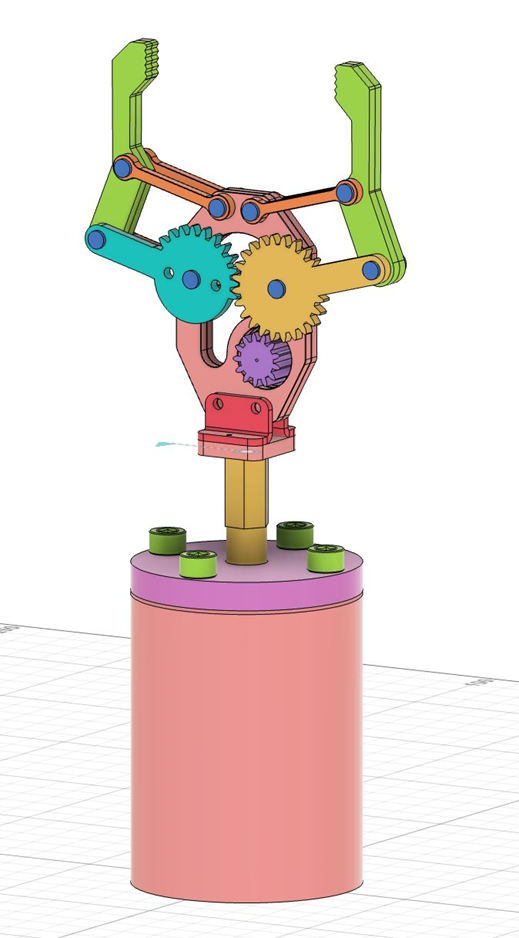
\includegraphics[width=0.6\linewidth]{Claw.png}
    \caption{Claw Model Design}
\end{figure}
\section{Subsystem Introduction}
\subsection{Digital Twins Subsystem}
\subsubsection*{Subsystem Description}
The Unity3D Digital Twin Subsystem provides a real-time 3D virtual replica of 
the physical system, using the Unity game engine to simulate and visualize the 
system's state. Its primary purpose is to mirror the physical equipment's 
behavior in a virtual environment for monitoring and operator interaction. 
The subsystem integrates Unity's physics engine and high-fidelity graphics 
rendering to model motions, forces, and object interactions that closely 
resemble the real world​. This digital twin receives live data from the physical 
system via a communication interface and updates the virtual model accordingly, 
thereby maintaining synchronization with the real equipment in near real-time. 
Within the overall system architecture, the Unity3D Digital Twin acts as the 
visualization and simulation layer. The Unity3D subsystem consumes these updates 
and applies them to the virtual model. In turn, the digital twin can also produce 
outputs or events​. This interaction enables scenarios like virtual commissioning 
and operator training, where the digital twin not only mirrors the physical 
system but can also influence it under controlled conditions. By leveraging 
Unity’s deployment, the digital twin visualization can run on operator VR 
headsets. 
\subsubsection*{Subsystem Requirements}
Real-Time Visualization Performance: The subsystem shall provide a smooth 
real-time visualization of the physical system. It must maintain a frame rate 
of at least 30 frames per second (FPS) during normal operation, with a target 
of 60 FPS for optimal smoothness.
  
Data Throughput and Update Rate: The Unity3D subsystem shall handle incoming 
data streams from the physical system at a sufficient rate. It must support at 
least 10 Hz update frequency for all critical sensor inputs, matching the data 
acquisition rate of the system​. 
  
Scene Complexity and Rendering Capability: The subsystem shall support the full 
complexity of the system's 3D model and environment. It must render all relevant 
components with high visual fidelity, including using imported CAD models for 
accuracy​. 
  
Integration and Compatibility: The Unity3D subsystem must integrate seamlessly 
with the overall system's data and control architecture. It shall support 
standard industrial communication protocols or APIs provided by the system 
integrator. 
\subsubsection*{Subsystem Verification}
Frame Rate Performance Test: Set up a full-scale virtual scene in Unity that 
represents the complete physical system. Run the digital twin application on 
the target hardware under typical operating conditions. Use Unity's built-in 
frame timing stats to record the frame rate. Verification criteria: The 
measured frame rate should stay ≥30 FPS for 95\% of the samples. 
  
Accuracy Validation Test: To verify the physical fidelity, we will compare 
the digital twin's reported state against the real system's state under 
controlled motions. We will record the corresponding position of the virtual 
model in Unity (the transform values or angles of the virtual joints). If a 
robot arm moves through 90°, the Unity twin's arm should be within range at 
all times. We will specifically check the worst-case alignment at extreme 
positions and dynamic moves. 
\subsection{VR Subsystem}
\subsubsection*{Subsystem Description}
The Meta Quest (or Oculus Quest VR headset) App block enables Meta Quest users to interact with the digital twin scene. In the runtime, it receives user hand trajectory from real world input. Then it processes the information for object recognition and finally sends the object index as well as the hand trajectory to the unity digital twin. 
\textbf{Input:}  
\begin{enumerate}
    \item \textbf{Predefined 3D Models and Configurations:} A set of digital models representing 10 objects, a table, and a robotic arm with an end-point gripper. These models are loaded at initialization.
    \item \textbf{Scale \& Spatial Arrangement Data:} Tolerances data ensuring that scale precision remains within less than a 5\% error margin and that objects are distinctly separated from the table.
\end{enumerate}
\textbf{Output:} 
\begin{enumerate}
    \item \textbf{Rendered Digital Twin Scene:} A virtual representation in Unity that mirrors the physical arrangement with the required precision. 
    \item \textbf{Visual Context Data:} The positioning data of each element (objects, table, robotic arm) used by the object recognition module to compare with user hand trajectories. 
\end{enumerate}
\subsubsection*{Subsystem Requirements}
$\bullet$ The predefined scene serves as a VR counterpart to our Digital Twin in Unity. It incorporates physical models of the following elements: 10 objects, table and robotic arm. 

 

\textbf{Requirements:} The elements in the scene must have less than 5\% precision tolerance in scales. The 10 objects must be viewed as separable entities from the table. The robotic arm could be simplified as a rigid body, but the end-point gripper must manifest the same level of detail with other elements. 

 

$\bullet$ Hands Tracking module captures user hands trajectories and sends them to the Digital Twin in Unity via proprietary API databus1 and object recognition module in real time. This is the key element to enable human robot interaction and is implemented by Unity First-Hand Dependencies \cite{unity-firsthand}. 

 

\textbf{Requirements:} Must capture hand trajectory every 0.2 seconds. Must convert the trajectory data to unity-readable format.
 
$\bullet$ Object Recognition module predicts which object the user is targeting based on hand trajectories and records the object is grasped. It constantly receives data from Hands Tracking module and reads the real-time object locations in the scene as input, and after processing it sends the “predicted\_object” data packet to the Digital Twin Unity via proprietary API databus 2. The prediction task is a classification problem on the 10 objects with input of a string of hand trajectory in the past 10 seconds. The code is written into Meta Quest App Build. 

 

\textbf{Requirement:} The classification task should be performed in a limited time, e.g. 0.2 seconds. The prediction result must be accurate as the user hand approaches close (within 10 cm) to the target object.  

 
\subsubsection*{Subsystem Verification}
\textbf{Scene Module:} 
\begin{enumerate}
    \item Validate that imported models maintain scale precision by running automated comparisons against defined dimensional tolerances. 
    \item Test that spatial relationships (i.e., object separability) are preserved. 
\end{enumerate}
 
\textbf{Hands Tracking:} 
\begin{enumerate}
    \item Simulate sensor inputs to ensure that trajectory data is sampled exactly every 0.2 seconds. 
    \item Check correct conversion routines by comparing raw sensor data to Unity-compatible data formats. 
\end{enumerate}
 
\textbf{Object Recognition:} 
\begin{enumerate}
    \item Use synthetic trajectory data covering typical usage (including cases when the hand is within 10 cm of an object) to verify that classification returns the correct object index. 
    \item Measure processing time to confirm that prediction completes within the 0.2-second window. 
\end{enumerate}
 
\textbf{Integrated Testing:}
\begin{enumerate}
    \item Simulate the digital twin in Unity to receive and correctly interpret both hand trajectory and object recognition outputs via their respective data buses (Databus1 and Databus2). 
    \item Introduce simulated delays or corrupted data in sensor inputs to verify that error handling protocols are initiated and logged. 
\end{enumerate}
\subsection{Mechanical Arm Subsystem}
\subsubsection*{Subsystem Description}
The mechanical claw subsystem serves as the end-effector of the UR3 robotic arm, designed to enhance its ability to grasp small and irregularly shaped objects. Unlike the original suction-based unit, the claw uses a servo motor for independent actuation and provides improved adaptability to non-flat surfaces. The claw body is fabricated from laser-cut acrylic plates and assembled with M3 screws and nuts, allowing for quick prototyping and ease of maintenance. The subsystem mounts directly onto the UR3 flange and receives PWM control signals from the upper-level controller, enabling precise open-close motions. End-stop feedback sensors can be optionally integrated to provide closed-loop control. 
\subsubsection*{Subsystem Requirements}
This subsystem is fully student-designed and must comply with dimensional, functional, and performance constraints: 
\begin{itemize}
    \item \textbf{Size:} The claw must remain compact to fit within the working envelope of the UR3. The maximum allowable dimensions are 12 cm (length) × 10 cm (width). 
    \item \textbf{Gripping Range:} The claw should be capable of grasping objects with widths ranging from 0.8 cm to 6 cm, covering a broad range of daily-use items such as pens, keys, and bottle caps. 
    \item \textbf{Gripping Force:} A minimum holding force of 1.5 N is required to securely lift lightweight objects (~150g), assuming a friction coefficient of 0.4 between the gripper and object surfaces. 
    \item \textbf{Positioning Accuracy:} The maximum allowable misalignment during gripping is ±0.5 cm, necessitating adequate structural rigidity and low mechanical backlash. 
    \item \textbf{Material: Lightweight} and rigid materials must be used to minimize added load on the robotic arm. The current prototype uses 4 mm-thick acrylic plates. 
\end{itemize}
\subsubsection*{Subsystem Verification}
To verify that the claw meets performance and usability standards, the following test procedures will be conducted: 
\begin{itemize}
    \item \textbf{Grasping Tests:} The claw will attempt to grasp 10 different objects varying in size (0.8\–5 cm), shape (cylindrical, cubic, irregular), surface texture (smooth/rough), and mass (30–150 g). 
    \item \textbf{Holding Stability:} Each object will be held stationary for 5 seconds post-grasp. Success is defined as no slippage or drop.     
    \item \textbf{Repeatability Test:} Each grasping action will be repeated 10 times, with a target success rate of ≥90\% to ensure consistent performance. 
    \item \textbf{Durability Check:} After 100 grasp-release cycles, structural integrity and gripping force will be reevaluated. 
\end{itemize}
\section{Tolerance Analysis}
\subsection{Power Supply}
\subsubsection{UR3 Robotic Arm}
The UR3 typically operates on a 24V DC power supply. The current drawn by the robotic arm varies depending on the motion and the load. Under typical operating conditions, the current draw can be around 3-6 A, which means the maximum power consumption can peak at around 150-200 W. We need to use a satisfied DC source or designed AC-DC converter. 
\subsubsection{STM32 Chip}
We will use STM32F4 series chips to control the claw motor, which needs a 5V DC voltage to power. Therefore, there should be a transformer before using the 6th signal of UR3 as input of STM32.  
\subsection{UR3 Precision}
There are limitations to robotic UR3, ensuring that it can accurately move 
following the computed route. Motivation speed is one of the most important 
factors. As mentioned in the instruction document, the general speed tolerance 
is -150mm/s. This means that if the user configures a 250mm/s speed limit, then 
the maximum operational speed will be 250-150=100mm/s. Safety tolerances 
prevent safety violations while allowing for fluctuations in program behavior. 
For example, when handling a heavy payload, there may be situations where the 
Robot Arm needs to briefly operate above the normal maximum operational speed to 
follow a programmed trajectory \cite{ur3-manual}. An example of such a situation is shown in 
figure. 
\begin{figure}[H]
    \centering
    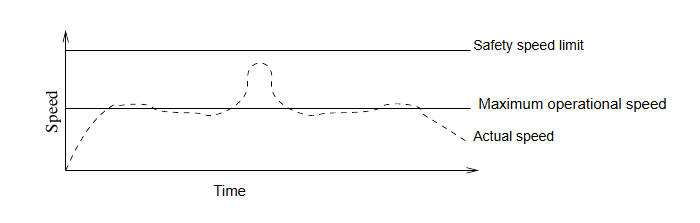
\includegraphics[width=0.8\linewidth]{UR3 Tolerance.png}
    \caption{Safety Tolerance Example}
\end{figure}
\subsection{Mechanical Claw}
A preliminary tolerance analysis focuses on the relationship between servo 
rotation and claw tip displacement. Based on linkage geometry, a ±$2^{\circ}$ servo 
error translates to approximately ±1.2 mm positional error at the gripper tips. 
The system’s performance is not highly sensitive to this variation, but finer 
control can be achieved by increasing servo resolution or using stiffer 
linkages. 
\subsection{Torch of Grasping}
The precision of grasping, especially whether the claw could successfully hold 
on to the items, mostly relies on the force of the claw applied. In other words, 
it depends on the torch range that the motor could supply. To verify the 
feasibility of our design, we want to use FEA ( Finite Element Analysis) 
method. Based on the shape, size, and material properties of the gripper’s 
fingers and the geometry of the object being grasped, combine this information 
with the 3D model of the claw to construct the model in FEA software, like 
ANSYS, COMSOL, or Abaqus. Use Static or Dynamic analysis to simulate contact 
pressure and displacement. With this information, we could get an appropriate 
torch. For example, the object material is plastic and can obtain 60 MPa 
maximum stress before damage. The friction coefficient ($\mu$) is 0.3. After 
simulation, we find we need to apply 15N force on the object, the contact area 
is $3mm^2$, according to the formula: 
\begin{equation*}
    Pressure(P)=\frac{Force(F)}{Area(S)}=\frac{15}{3} \cdot 10^{-6}=5MPa<60MPa 
\end{equation*}

We could ensure claw will not break the object if grasped successfully. Therefore, we could compute the corresponding Torch(T) with formula: 
\begin{equation*}
    Torch(T)=Length(L) \times Force(F)
\end{equation*} 
\chapter{Cost \& Schedule}
\section{Cost Analysis}
\begin{table}[H]
    \centering
    \caption{Example of a Table and Its Title}
    \label{Cost-table}
    \begin{tabular}{@{}c|cc@{}}
        \toprule
        Part                & Electricity  & Magnetism \\ \midrule
        Field intensity     & $E$          & $H$       \\
        Flux density        & $D$          & $B$       \\
        Constitutive factor & $\epsilon^b$ & $\mu$     \\ \bottomrule
    \end{tabular}
\end{table}
\section{Schedule}
An example piece of inserting code from an existing file.
\chapter{Ethics \& Safety}
%%%%%%%%%%%%%%%%%%%%%%%%%%%%%%%%%%%%%%%%%%%%%%%%%%%%%%%%%%%%%%%%%

%%% Appendices %%%%%%%%%%%%%%%%%%%%%%%%%%%%%%%%%%%%%%%%%%%%%%%%%%
\titleformat{\chapter}
{\fontsize{16pt}{\baselineskip}\selectfont\bfseries}
{Appendix \thechapter}{1em}{}
\titlespacing{\chapter}{0pt}{0pt}{\baselineskip}
% \begin{appendices}
%     % All appendices here, using sections for multiple appendices
%     \chapter{Requirement and Verification Table}
%     An appendix is a good place for the Requirement and Verification Table from your design review. Below is a starter table. Including these details here will help to avoid lengthy and tedious narrative descriptions in the main text, which may not be of immediate interest to your imagined audience of company managers and professionals. Any requirement that is not verified should be explained either in the main text or the appendix. Note that both the pagination and the numbering of figures, tables, and equations continue from the main text to the appendices.

%     Tab. \ref{tab:srv} is generated by Excel2LaTeX. See \url{https://www.ctan.org/tex-archive/support/excel2latex/} for more details.
%     % Table generated by Excel2LaTeX from sheet 'Sheet1'
%     \begin{table}[htbp]
%         \centering
%         \caption{System Requirements and Verifications}
%         \begin{tabularx}{\textwidth}{X|X|c}
%             \toprule
%             \centering\multirow{2}[2]{*}{Requirement} & \centering\multirow{2}[2]{*}{Verification} & \multicolumn{1}{c}{Verification status} \\
%             \multicolumn{1}{c|}{}                     & \multicolumn{1}{c|}{}                      & \multicolumn{1}{c}{(Y or N)}                     \\
%             \midrule
%             1. Requirement                            & 1. Verification                            & \multirow{4}[1]{*}{}                             \\
%             a. Subrequirement                         & a. Subverification                         &                                                  \\
%             b. Subrequirement                         & b. Subverification                         &                                                  \\
%             c. Subrequirement                         & c. Subverification                         &                                                  \\\hline
%             2. Requirement                            & 2. Verification                            & \multirow{4}[0]{*}{}                             \\
%             a. Subrequirement                         & a. Subverification                         &                                                  \\
%             b. Subrequirement                         & b. Subverification                         &                                                  \\
%             c. Subrequirement                         & c. Subverification                         &                                                  \\\hline
%             3.                                        & 3.                                         &                                                  \\\hline
%             4.                                        & 4.                                         &                                                  \\\bottomrule
%         \end{tabularx}%
%         \label{tab:srv}%
%     \end{table}%

%     \section{Some Test Data}
% \end{appendices}
\titleformat{\chapter}
{\fontsize{16pt}{\baselineskip}\selectfont\bfseries}
{\thechapter}{1em}{}
\titlespacing{\chapter}{0pt}{0pt}{\baselineskip}
\clearpage
%%%%%%%%%%%%%%%%%%%%%%%%%%%%%%%%%%%%%%%%%%%%%%%%%%%%%%%%%%%%%%%%%
\backmatter
%%% References %%%%%%%%%%%%%%%%%%%%%%%%%%%%%%%%%%%%%%%%%%%%%%%%%%
\clearpage
\renewcommand*{\UrlFont}{\rmfamily}
\printbibliography[title={References},heading=bibintoc]
\clearpage
%%%%%%%%%%%%%%%%%%%%%%%%%%%%%%%%%%%%%%%%%%%%%%%%%%%%%%%%%%%%%%%%%
\end{document}